\subsection{Codificadores e protocolo de treinamento}
\label{sec:modelos}

Os modelos (Figura~\ref{fig:arquitetura}) projetam os \num{17} atributos $\mathbf{f}_i$ de cada nó num estado inicial $\mathbf{h}_i^{(0)}$ de largura $D$ e aplicam $L = {}$\num{4} camadas residuais,
\begin{equation}
  \mathbf{h}_i^{(\ell)} = \mathbf{h}_i^{(\ell-1)} + \mathrm{GELU}\Big(\mathrm{Conv}^{(\ell)}\big(\mathrm{LN}^{(\ell)}(\mathbf{h}_i^{(\ell-1)}),\ \{(\mathrm{LN}^{(\ell)}(\mathbf{h}_j^{(\ell-1)}),\, \mathbf{e}_{ji})\}_{j \in \mathcal{N}(i)}\big)\Big), \quad \ell = 1, \dots, L,
  \label{eq:camada}
\end{equation}
com normalização de camada $\mathrm{LN}^{(\ell)}$ de \citeonline{ba2016layer}, ativação GELU (unidade linear de erro gaussiano) de \citeonline{hendrycks2016gaussian} e operador $\mathrm{Conv}^{(\ell)}$, que lê $\mathbf{e}_{ji}$, exceto em EdgeConv, GraphSAGE e ResGatedGCN. Nos GPS, uma porta aprendida mistura um GATv2 local, sem GELU, e uma atenção global; um bloco denso residual completa a camada. A leitura concatena média, máximo e soma comprimida por logaritmo dos estados. Os \num{33} escalares $\mathbf{u}$ entram na cabeça de regressão diretamente e também codificados em \num{128} dimensões. A cabeça prevê $x$, depois $y$ dado o $x$ previsto e $z$ dados os $x$ e $y$ previstos, mesmo no treino, por modulação linear por atributo (FiLM) de \citeonline{perez2018film} ou, nos modelos de sufixo cascata, por concatenação; o sufixo designa só a cabeça. Uma limitação suave mantém a predição na caixa \textpm(\num{6.03};~\num{6.67};~\num{29.93})\,\unit{\m}, com inclinação pequena fora dela.

\begin{figure}[H]
  \centering
  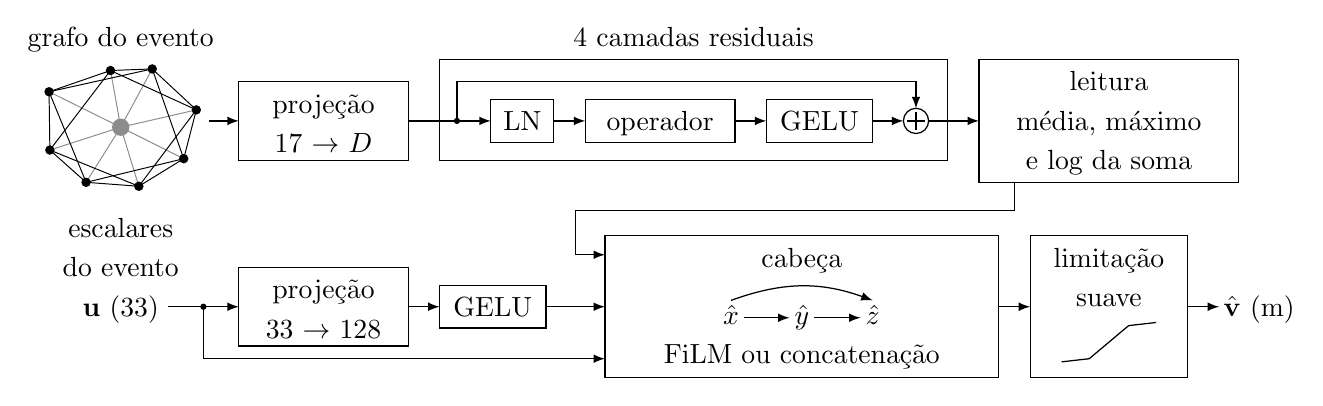
\begin{tikzpicture}[
  x=1cm, y=1cm,
  line width=0.45pt,
  flow/.style={-latex, line width=0.45pt},
  knn/.style={line width=0.35pt},
  spoke/.style={line width=0.35pt, draw=black!45},
  channel/.style={circle, fill=black, inner sep=0pt, minimum size=1.2mm},
  globalnode/.style={circle, fill=black!45, inner sep=0pt, minimum size=2.2mm},
  branch/.style={circle, fill=black, inner sep=0pt, minimum size=0.8mm},
  txt/.style={inner sep=0pt, anchor=base},
  dag/.style={inner sep=1.6pt, execute at begin node={\vphantom{$\hat{x}\hat{y}\hat{z}$}}}
]
\def\arqrowa{3.28}
\def\arqrowb{0.92}
\def\arqgap{2.14}
\def\arqtop{4.22}

\coordinate (g)  at (1.45, 3.20);
\coordinate (c0) at (2.41, 3.42);
\coordinate (c1) at (1.85, 3.94);
\coordinate (c2) at (1.32, 3.92);
\coordinate (c3) at (0.54, 3.65);
\coordinate (c4) at (0.55, 2.91);
\coordinate (c5) at (1.01, 2.50);
\coordinate (c6) at (1.68, 2.45);
\coordinate (c7) at (2.25, 2.80);

\foreach \i in {0,...,7} {\draw[spoke] (g) -- (c\i);}
\foreach \i/\j in {0/1,1/2,2/3,3/4,4/5,5/6,6/7,7/0,0/2,1/3,2/4,3/5,4/6,5/7,6/0,7/1} {\draw[knn] (c\i) -- (c\j);}
\foreach \i in {0,...,7} {\node[channel] at (c\i) {};}
\node[globalnode] at (g) {};
\node[txt] at (1.45, \arqtop) {grafo do evento};

\draw[flow] (2.57, \arqrowa) -- (2.95, \arqrowa);
\draw (2.95, \arqrowa-0.50) rectangle (5.10, \arqrowa+0.50);
\node[txt] at (4.025, \arqrowa+0.10) {projeção};
\node[txt] at (4.025, \arqrowa-0.40) {\num{17} $\to$ $D$};

\draw (5.50, \arqrowa-0.50) rectangle (11.95, \arqrowa+0.78);
\node[txt] at (8.725, \arqtop) {\num{4} camadas residuais};
\draw[flow] (5.10, \arqrowa) -- (6.15, \arqrowa);
\node[branch] at (5.72, \arqrowa) {};
\draw[flow] (5.72, \arqrowa) -- (5.72, \arqrowa+0.50) -- (11.55, \arqrowa+0.50) -- (11.55, \arqrowa+0.16);
\draw (6.15, \arqrowa-0.27) rectangle (6.95, \arqrowa+0.27);
\node[txt] at (6.55, \arqrowa-0.12) {LN};
\draw[flow] (6.95, \arqrowa) -- (7.35, \arqrowa);
\draw (7.35, \arqrowa-0.27) rectangle (9.25, \arqrowa+0.27);
\node[txt] at (8.30, \arqrowa-0.12) {operador};
\draw[flow] (9.25, \arqrowa) -- (9.65, \arqrowa);
\draw (9.65, \arqrowa-0.27) rectangle (11.00, \arqrowa+0.27);
\node[txt] at (10.325, \arqrowa-0.12) {GELU};
\draw[flow] (11.00, \arqrowa) -- (11.39, \arqrowa);
\draw (11.55, \arqrowa) circle (0.16);
\draw (11.44, \arqrowa) -- (11.66, \arqrowa);
\draw (11.55, \arqrowa-0.11) -- (11.55, \arqrowa+0.11);
\draw[flow] (11.71, \arqrowa) -- (12.35, \arqrowa);

\draw (12.35, \arqrowa-0.78) rectangle (15.65, \arqrowa+0.78);
\node[txt] at (14.00, \arqrowa+0.38) {leitura};
\node[txt] at (14.00, \arqrowa-0.12) {média, máximo};
\node[txt] at (14.00, \arqrowa-0.62) {e log da soma};

\draw[flow] (12.80, \arqrowa-0.78) -- (12.80, \arqgap) -- (7.225, \arqgap) -- (7.225, \arqrowb+0.66) -- (7.60, \arqrowb+0.66);

\node[txt] at (1.45, \arqrowb+0.88) {escalares};
\node[txt] at (1.45, \arqrowb+0.38) {do evento};
\node[txt] at (1.45, \arqrowb-0.12) {$\mathbf{u}$ (\num{33})};
\draw[flow] (2.05, \arqrowb) -- (2.95, \arqrowb);
\node[branch] at (2.50, \arqrowb) {};
\draw[flow] (2.50, \arqrowb) -- (2.50, \arqrowb-0.66) -- (7.60, \arqrowb-0.66);
\draw (2.95, \arqrowb-0.50) rectangle (5.10, \arqrowb+0.50);
\node[txt] at (4.025, \arqrowb+0.10) {projeção};
\node[txt] at (4.025, \arqrowb-0.40) {\num{33} $\to$ \num{128}};
\draw[flow] (5.10, \arqrowb) -- (5.50, \arqrowb);
\draw (5.50, \arqrowb-0.27) rectangle (6.85, \arqrowb+0.27);
\node[txt] at (6.175, \arqrowb-0.12) {GELU};
\draw[flow] (6.85, \arqrowb) -- (7.60, \arqrowb);

\draw (7.60, \arqrowb-0.90) rectangle (12.60, \arqrowb+0.90);
\node[txt] at (10.10, \arqrowb+0.50) {cabeça};
\node[dag] (xh) at (9.20, \arqrowb-0.14) {$\hat{x}$};
\node[dag] (yh) at (10.10, \arqrowb-0.14) {$\hat{y}$};
\node[dag] (zh) at (11.00, \arqrowb-0.14) {$\hat{z}$};
\draw[flow] (xh) -- (yh);
\draw[flow] (yh) -- (zh);
\draw[flow] (xh.north) to[bend left=20] (zh.north);
\node[txt] at (10.10, \arqrowb-0.72) {FiLM ou concatenação};
\draw[flow] (12.60, \arqrowb) -- (13.00, \arqrowb);

\draw (13.00, \arqrowb-0.90) rectangle (15.00, \arqrowb+0.90);
\node[txt] at (14.00, \arqrowb+0.50) {limitação};
\node[txt] at (14.00, \arqrowb) {suave};
\draw (13.40, \arqrowb-0.70) -- (13.75, \arqrowb-0.66) -- (14.25, \arqrowb-0.24) -- (14.60, \arqrowb-0.20);
\draw[flow] (15.00, \arqrowb) -- (15.40, \arqrowb);
\node[txt, anchor=base west] at (15.45, \arqrowb-0.12) {$\hat{\mathbf{v}}$ (m)};
\end{tikzpicture}\relax

  \caption{Estrutura comum aos \num{11} codificadores. O grafo do evento tem um nó por canal ativo e um nó global no centroide da luz; quatro camadas residuais atualizam os estados dos nós, que a leitura resume em média, máximo e soma comprimida por logaritmo; a cabeça recebe também os \num{33} escalares do evento e prevê $x$, depois $y$ dado o $x$ previsto ($\hat{x}$) e $z$ dados $\hat{x}$ e o $y$ previsto ($\hat{y}$); a limitação suave mantém o vértice previsto $\hat{\mathbf{v}}$, em metros, na caixa definida pelos canais. Entre os codificadores mudam só o operador (nos GPS, a camada inteira), a largura $D$ e, nos modelos de sufixo cascata, a cabeça.}
  \label{fig:arquitetura}
\end{figure}

A largura $D$ de cada codificador foi escolhida \cite{dwivedi2023benchmarking} para aproximar o total de parâmetros do GPS, \num{1843395}. Dos \num{14} codificadores dimensionados, \num{11} foram treinados (Seção~\ref{sec:dificuldades}), com \num{1819019} a \num{1873531} parâmetros (desvio máximo de \qty{1.6}{\percent}) e $D$ de \num{132} a \num{685}, exceto no GPS (Tabela~\ref{tab:codificadores}). A capacidade equiparada é a do modelo inteiro: a parcela do codificador vai de \qty{58.3}{\percent} (EdgeConv) a \qty{85.4}{\percent} (\mbox{GPS-cascata}).

A perda $\mathcal{L}$ é a distância euclidiana média, em metros, entre o vértice previsto $\hat{\mathbf{v}}_b$ e o verdadeiro $\mathbf{v}_b$ das $B$ linhas $b$ do lote,
\begin{equation}
  \mathcal{L} = \frac{1}{B} \sum_{b=1}^{B} \big\lVert \hat{\mathbf{v}}_b - \mathbf{v}_b \big\rVert,
  \label{eq:perda}
\end{equation}
a mesma grandeza do erro 3-D médio. O otimizador AdamW \cite{loshchilov2019decoupled} usou coeficientes das médias móveis de \num{0.9} e \num{0.999}, decaimento de pesos de \num{e-4} no codificador e \num{e-5} na cabeça, e taxas de aprendizado de \num{5e-4} e \num{5e-3}, respectivamente, para lotes de \num{128} (\num{1.5e-4} e \num{1.5e-3} nos GPS), multiplicadas por $B$/\num{128} \cite{goyal2017accurate}. O lote $B$ foi a maior potência de dois, até \num{512}, que coube em \qty{20}{\gibi\byte} numa sonda de memória: \num{128} em quatro modelos, \num{256} em dois e \num{512} em cinco. Houve aquecimento linear de \num{100} passos de otimização a partir de \num{0.1} vez a taxa, decaimento cossenoidal até \num{e-6} em \num{50} épocas \cite{loshchilov2017sgdr} e limitação da norma do gradiente em \num{1.0}. O teste usou o ponto de verificação de menor erro de validação; não houve precisão mista, aumento de dados além do espelhamento nem média móvel dos pesos. Cada codificador foi treinado uma vez, com semente \num{42}, sem busca de hiperparâmetros. Os treinos somaram \qty{11.42}{\hour} numa unidade de processamento gráfico (GPU) de \qty{23.98}{\gibi\byte}, com \num{5600} a \num{22250} passos: a capacidade foi equiparada, mas o orçamento de otimização variou.
